%
% teil3.tex -- Resultate und Ausblick
%
% (c) 2022 Fabian Dünki, Hochschule Rapperswil
%
\section{Auswertung
\label{0f1:section:teil3}}
\rhead{Resultate}
Im Verlauf des Seminares hat sich gezeigt, 
das ein einfacher mathematischer Algorithmus zu implementieren gar nicht so einfach ist.
So haben alle drei umgesetzten Ansätze Probleme mit grossen negativen $z$ in der Funktion $\mathstrut_0F_1(;c;z)$.
Ebenso kann festgestellt werden,dass je grösser der Wert $z$ in $\mathstrut_0F_1(;c;z)$ wird, desto mehr weichen die berechneten Resultate von den Erwarteten ab. \cite{0f1:wolfram-0f1}

\subsection{Konvergenz
\label{0f1:subsection:konvergenz}}
Es zeigt sich in Abbildung \ref{0f1:ausblick:plot:airy:konvergenz}, dass schon nach drei Iterationen ($k = 3$) die Funktionen schon genaue Resultate im Bereich von -2 bis 2 liefert. Ebenso kann festgestellt werden, dass der Kettenbruch schneller konvergiert und im positiven Bereich sogar mit der Referenzfunktion $Ai(x)$ übereinstimmt. Da die Rekursionsformel \ref{0f1:listing:kettenbruchRekursion} eine Abwandlung des Kettenbruches ist, verhalten sich die Funktionen in diesem Fall gleich.

Erst wenn mehrere Durchläufe gemacht werden, um die Genauigkeit zu verbessern, ist der Kettenbruch den anderen zwei Algorithmen, bezüglich Konvergenz überlegen. 
Interessant ist auch, dass die Rekursionsformel nahezu gleich schnell wie die Potenzreihe konvergiert, aber sich danach einschwingt. Dieses Verhalten ist auch bei grösseren $z$ zu beobachten, allerdings ist dann die Differenz zwischen dem ersten lokalen Minimum von k bis zum Abbruch kleiner.
\ref{0f1:ausblick:plot:konvergenz:positiv}
Dieses Phänomen ist auf die Lösung der Rekursionsformel zurück zu führen.\ref{0f1:math:loesung:eq} Da im Gegensatz die ganz kleinen Werte nicht zu einer Konvergenz wie beim Kettenbruch führen, sondern sich noch eine Zeit lang durch die Multiplikation aufschwingen.

Ist $z$ negativ wie im Abbild \ref{0f1:ausblick:plot:konvergenz:negativ}, führt dies zu einer Gegenseitigen Kompensation von negativen und positiven Termen so bricht die Rekursionsformel hier zusammen mit der Potenzreihe ab.
Die ansteigende Differenz mit anschliessender, ist aufgrund der sich alternierenden Termen mit wechselnden Vorzeichens zu erklären.

\subsection{Stabilität
\label{0f1:subsection:Stabilitaet}}
Verändert sich der Wert von z in $\mathstrut_0F_1(;c;z)$ gegen grössere positive Werte, wie zum Beispiel $c = 800$ liefert die Kettenbruch-Funktion \ref{0f1:listing:kettenbruchIterativ} \verb+inf+ zurück. Dies könnte durch ein Abbruchkriterien abgefangen werden. Allerdings würde das, bei grossen Werten zulasten der Genauigkeit gehen. Trotzdem könnte, je nach Anwendung, auf ein paar Nachkommastellen verzichtet werden.

Wohingegen die Potenzreihe \ref{0f1:listing:potenzreihe} das Problem hat, dass je mehr Terme berechnet werden, desto schneller wächst die Fakultät und irgendwann gibt es eine Bereichsüberschreitung von \verb+double+. Schlussendlich gibt das Unterprogramm das Resultat \verb+-nan(ind)+ zurück.
Die Rekursionformel \ref{0f1:listing:kettenbruchRekursion} liefert für sehr grosse positive Werte die genausten Ergebnisse, verglichen mit der GNU Scientific Library. Wie schon vermutet ist die Rekursionsformel, im positivem Bereich, der stabilste Algorithmus. Um die Stabilität zu gewährleisten, muss wie in \ref{0f1:ausblick:plot:konvergenz:positiv} dargestellt, die Iterationstiefe $k$ genug gross gewählt werden.

Im negativem Bereich sind alle gewählten und umgesetzten Ansätze instabil. Grund dafür ist die Fakultät im Nenner, was zum Phänomen der Auslöschung führt.\cite{0f1:SeminarNumerik} Schön zu beobachten ist dies in der Abbildung \ref{0f1:ausblick:plot:airy:stabilitaet} mit der Airy-Funktion als Test. So sind sowohl der Kettenbruch, als auch die Rekursionsformel bis ungefähr $\frac{-15^3}{9}$ stabil. Dies macht auch Sinn, da beide auf der gleichen mathematischen Grundlage basieren. Danach verhält sich allerdings die Instabilität unterschiedlich. Das unterschiedliche Verhalten kann damit erklärt werden, dass beim Kettenbruch jeweils eine zusätzliche Division stattfindet. Diese Unterschiede sind auch in Abbildung \ref{0f1:ausblick:plot:konvergenz:positiv} festzustellen.



\begin{figure}
    \centering
    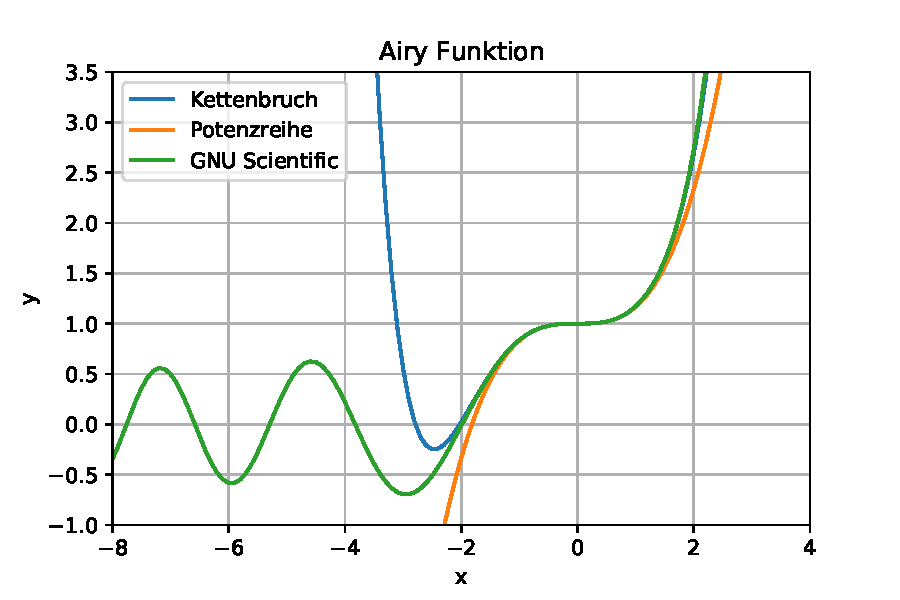
\includegraphics[width=0.8\textwidth]{papers/0f1/images/konvergenzAiry.pdf}
    \caption{Konvergenz nach drei Iterationen, dargestellt anhand der Airy Funktion zu den Anfangsbedingungen $Ai(0)=1$ und $Ai'(0)=0$.
    \label{0f1:ausblick:plot:airy:konvergenz}}
\end{figure}

\begin{figure}
    \centering
    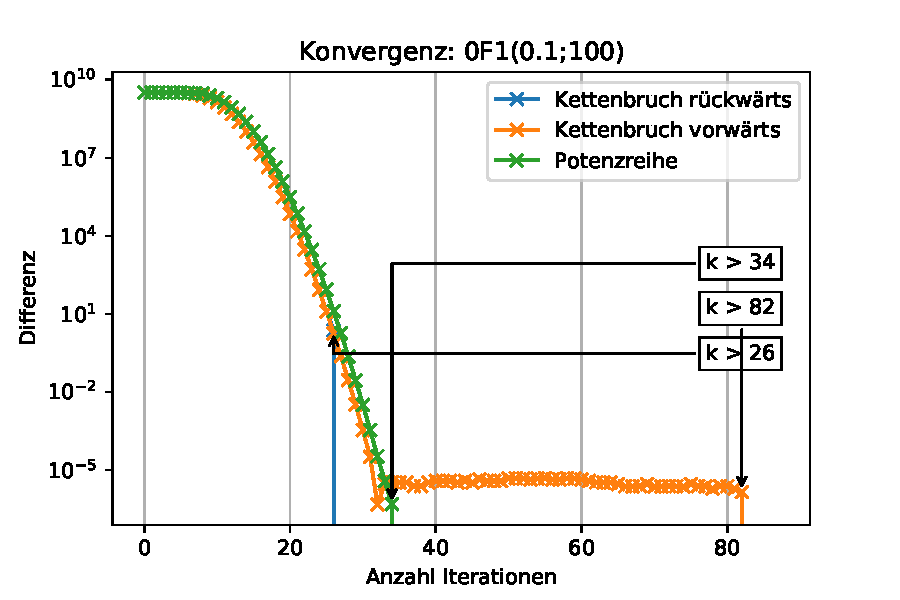
\includegraphics[width=0.8\textwidth]{papers/0f1/images/konvergenzPositiv.pdf}
    \caption{Konvergenz: Logarithmisch dargestellte Differenz vom erwarteten Endresultat.
    \label{0f1:ausblick:plot:konvergenz:positiv}}
\end{figure}

\begin{figure}
    \centering
    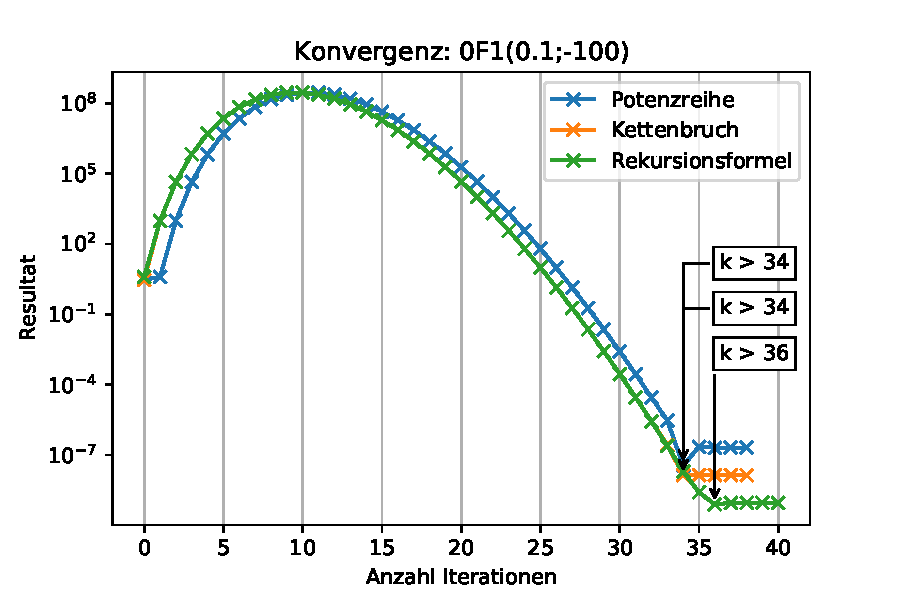
\includegraphics[width=0.8\textwidth]{papers/0f1/images/konvergenzNegativ.pdf}
    \caption{Konvergenz: Logarithmisch dargestellte Differenz vom erwarteten Endresultat.
    \label{0f1:ausblick:plot:konvergenz:negativ}}
\end{figure}

\begin{figure}
    \centering
    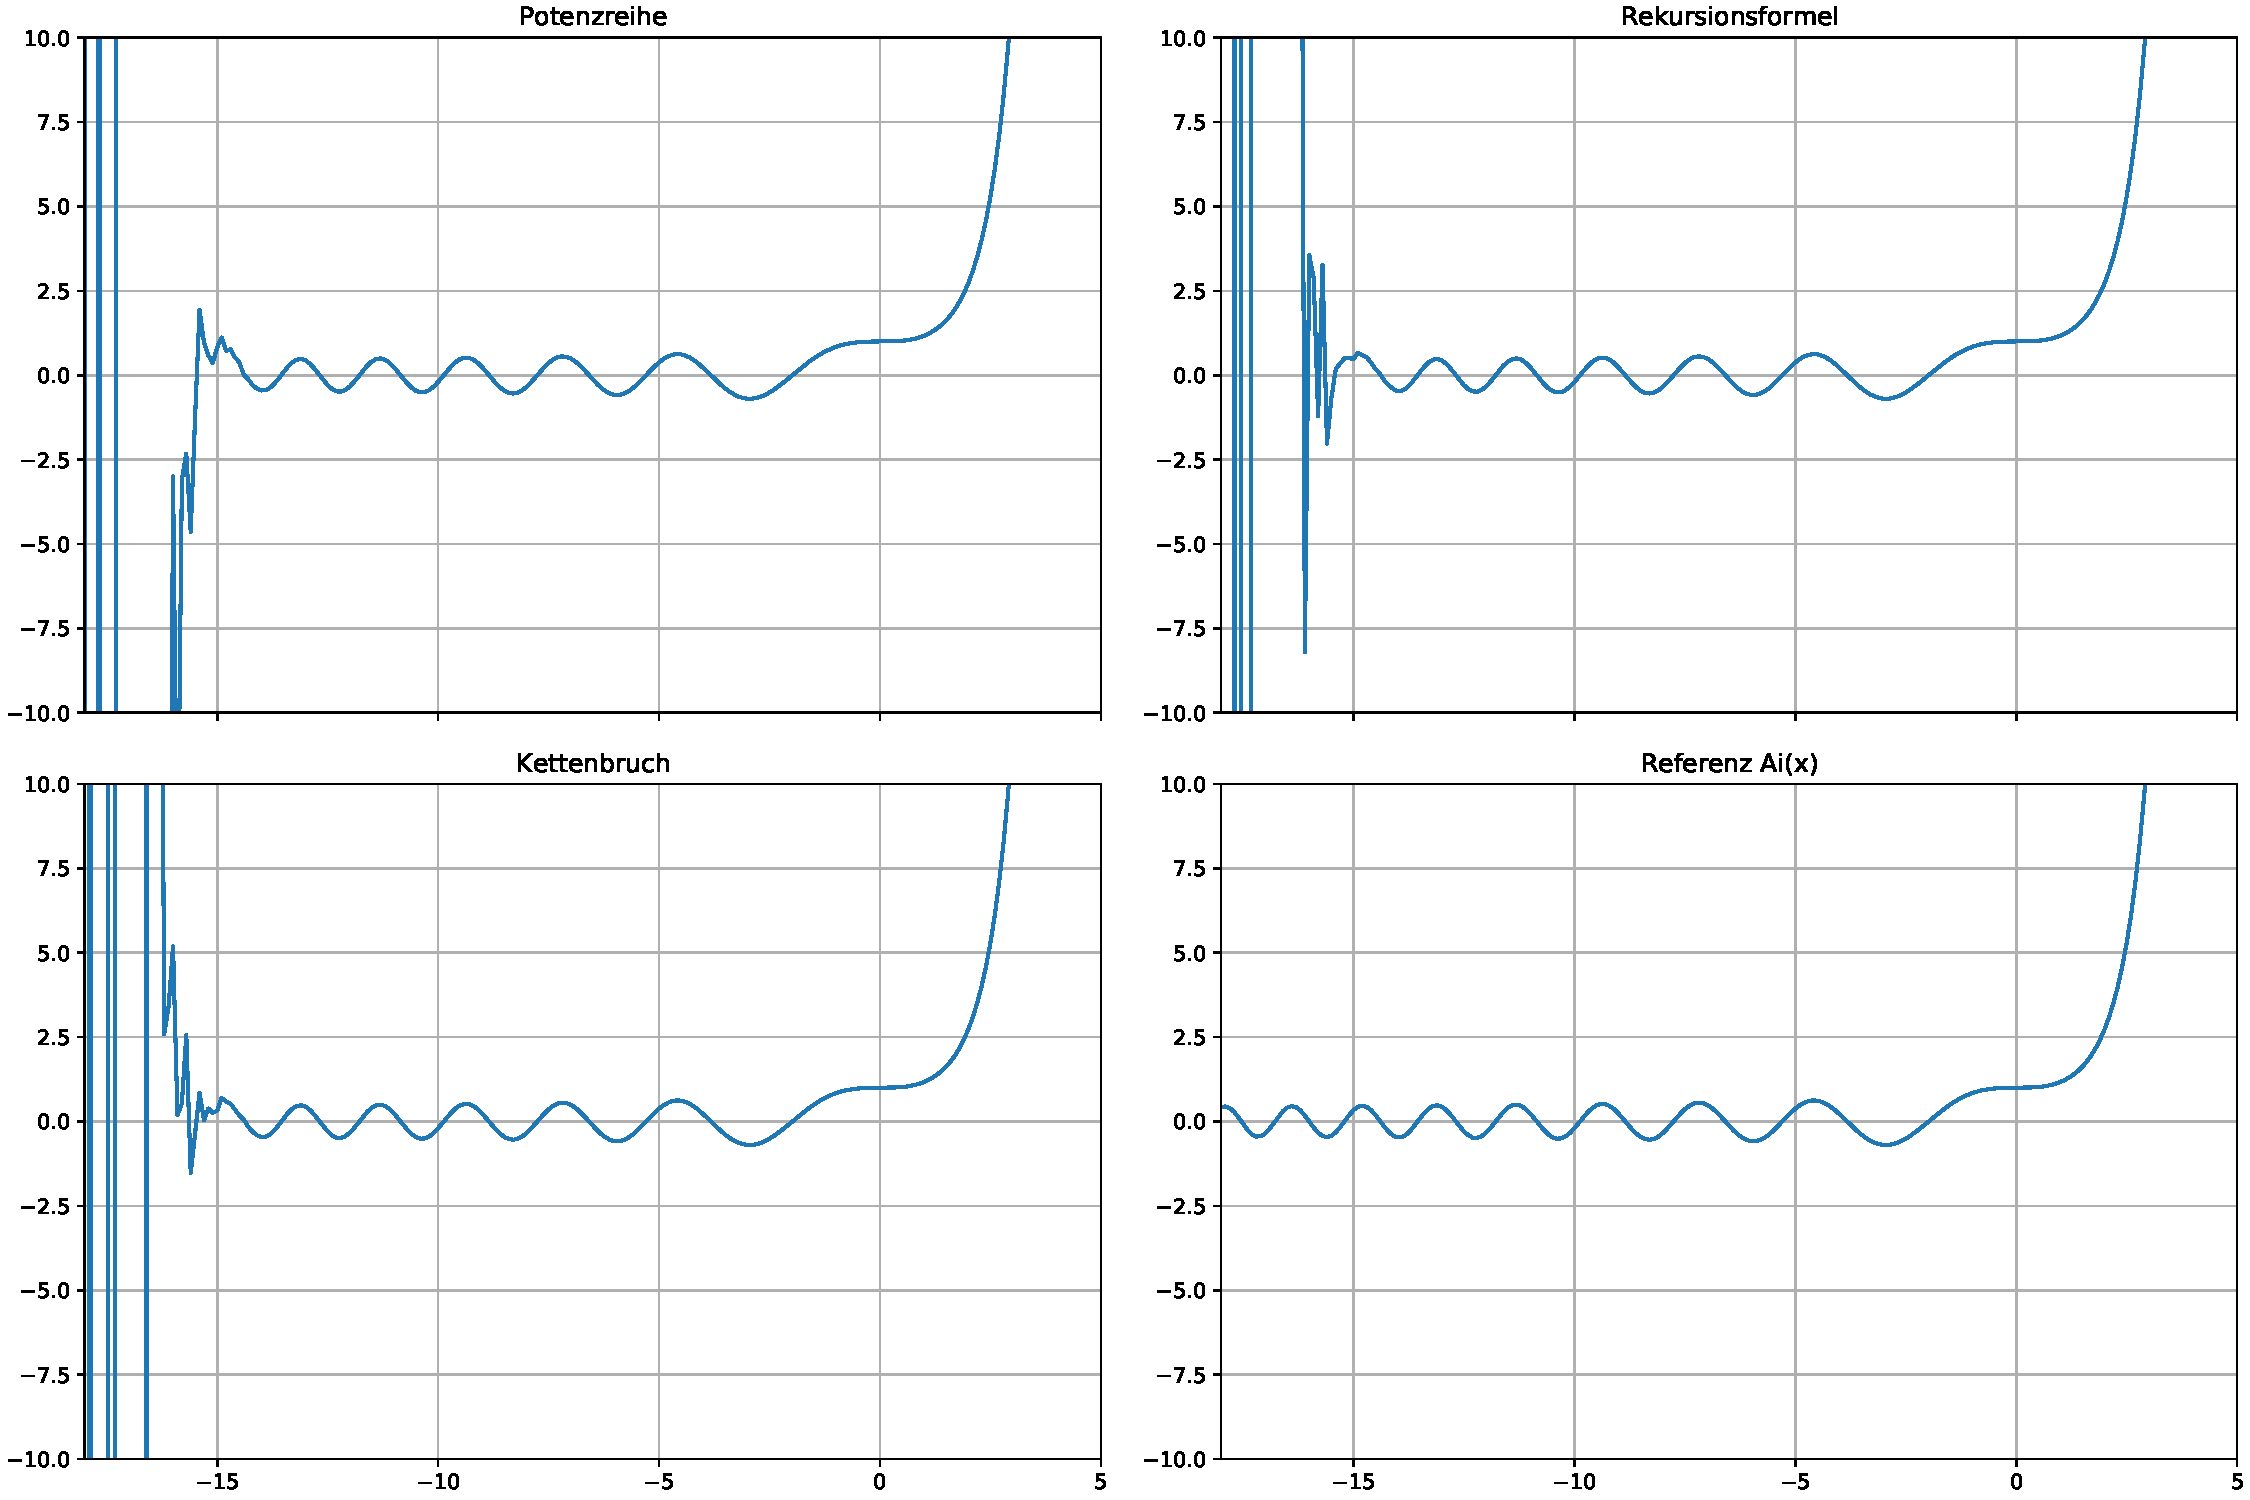
\includegraphics[width=1\textwidth]{papers/0f1/images/stabilitaet.pdf}
    \caption{Stabilität der 3 Algorithmen verglichen mit der Referenz Funktion $Ai(x)$.
    \label{0f1:ausblick:plot:airy:stabilitaet}}
\end{figure}

